\section{Results}
\label{sec:results}

\subsection{The DFT-informed pipeline versus the leaderboard (run 2)}
Table~\ref{tab:a2leader} and Fig.~\ref{fig:a2} compare the frozen run-2 pipeline with each task's leader.

\paragraph{expt\_gap}
The MAE is \AtwoFinalGap{}~eV against \AtwoLeaderGap{}~eV for Darwin. The difference is $\Delta=\AtwoDeltaGap$~eV (95\% CI [\AtwoCIloGap, \AtwoCIhiGap]; \AtwoPHolmExprGap). This is the only task that meets our pre-registered rule for beating the leader.

\paragraph{expt\_is\_metal and steels}
The pipeline is statistically on par with the leaders:
\begin{itemize}
\item expt\_is\_metal: balanced accuracy \AtwoFinalMetal{} versus \AtwoLeaderMetal{} (\AtwoPHolmExprMetal);
\item steels: MAE \AtwoFinalSteels{} versus \AtwoLeaderSteels~MPa (\AtwoPHolmExprSteels).
\end{itemize}

\paragraph{glass}
The pipeline is clearly behind MODNet v0.1.12: \AtwoFinalGlass{} versus \AtwoLeaderGlass{} (\AtwoPHolmExprGlass). This also holds for the probability ROC-AUC (\AtwoAUCGlass{} versus \AtwoLeaderAUCGlass).

\paragraph{Caveat}
These are not like-for-like comparisons. Our pipeline uses an external DFT block for expt\_gap and expt\_is\_metal, and the leaders did not (Section~\ref{sec:discussion}).

\begin{table}[t]
\centering
\caption{Run-2 (Amendment-2) final pipeline versus each task's leaderboard leader, paired over the official test compositions using the leaders' public per-sample predictions. Metrics follow the board: MAE; balanced accuracy for classification. $\Delta$ is ours minus the leader. 95\% CI: paired bootstrap over test points within folds. Holm correction over four tasks. Rank is among the entries of 18 October 2026, including ours.}
\label{tab:a2leader}
\begin{adjustbox}{max width=\textwidth}
\begin{tabular}{llccccc}
\toprule
Task & Metric & Final pipeline & Leader (board) & $\Delta$ [95\% CI] & $p_\mathrm{Holm}$ & Rank \\
\midrule
steels & MAE & 80.10 $\pm$ 10.19 & TPOT-Mat: 79.95 & +0.1577 [-4.54, +4.89] & 0.928 & 2 of 12 \\
expt\_gap & MAE & 0.2352 $\pm$ 0.0167 & Darwin: 0.2865 & -0.05131 [-0.0701, -0.0331] & $<$0.001 & 1 of 13 \\
expt\_is\_metal & bal.\ acc. & 0.9547 $\pm$ 0.0033 & Darwin: 0.9598 & -0.005093 [-0.0118, +0.00179] & 0.299 & 2 of 8 \\
glass & bal.\ acc. & 0.8937 $\pm$ 0.0158 & MODNet (v0.1.12): 0.9603 & -0.06658 [-0.0759, -0.0573] & $<$0.001 & 2 of 8 \\
\bottomrule
\end{tabular}

\end{adjustbox}
\end{table}

\begin{figure}[t]
\centering
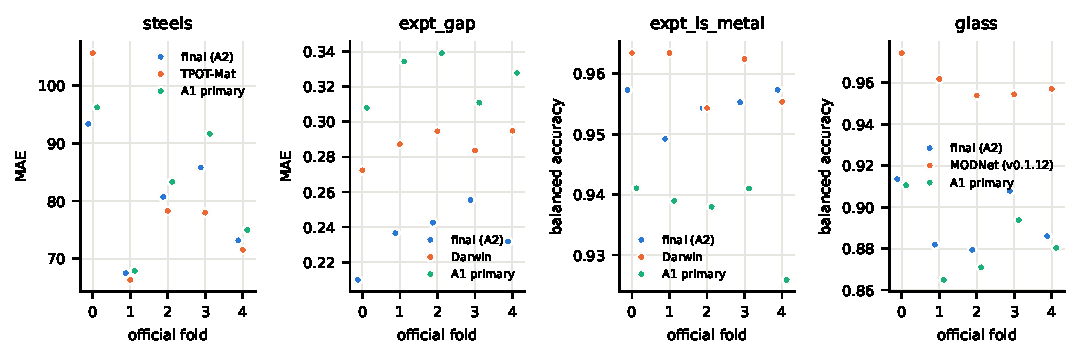
\includegraphics[width=\textwidth]{figures/fig_a2_leader.pdf}
\caption{Per-fold board metric of the run-2 final pipeline, the task leader and the run-1 primary arm.}
\label{fig:a2}
\end{figure}

\subsection{Where the gain comes from: post-hoc ablation}
The ablation in Table~\ref{tab:ablation} was written after run~2 had been scored and was not used for any selection; the reported pipeline is unchanged. It re-runs the frozen run-2 code, either without the DFT block (all tasks) or without the hurdle experts (expt\_gap).

\paragraph{expt\_gap}
\begin{itemize}
\item Without the DFT block, the MAE rises to \AblNoDftGap{}~eV (\AblNoDftGapRel\% relative to the full pipeline, $p_\mathrm{boot}=\AblNoDftGapP$).
\item Without the hurdle experts, it rises to \AblNoHurdleGap{}~eV (\AblNoHurdleGapRel\%, $p_\mathrm{boot}=\AblNoHurdleGapP$).
\end{itemize}

\paragraph{expt\_is\_metal}
Removing the DFT block changes the balanced accuracy to \AblNoDftMetal{} (\AblNoDftMetalRel\%, $p_\mathrm{boot}=\AblNoDftMetalP$).

\paragraph{glass and steels}
The DFT block matches few or none of the compositions on these tasks, and removing it changes little:
\begin{itemize}
\item glass: \AblNoDftGlassRel\%;
\item steels: \AblNoDftSteelsRel\%.
\end{itemize}

\begin{table}[t]
\centering
\caption{Post-hoc ablation of the frozen run-2 pipeline (plan Section~12; not used for selection). Board metric of the run-2 final pipeline and of each variant; paired bootstrap of the difference; number of folds in which the variant is worse; the leader's value, with the $p$-value of the variant versus the leader.}
\label{tab:ablation}
\begin{adjustbox}{max width=\textwidth}
\begin{tabular}{lllcccccccc}
\toprule
 & & & \multicolumn{2}{c}{mean $\pm$ s.d.\ over 5 folds} & \multicolumn{3}{c}{variant $-$ full A2} & \multicolumn{3}{c}{variant $-$ leader} \\
\cmidrule(lr){4-5}\cmidrule(lr){6-8}\cmidrule(lr){9-11}
Task & Metric & Variant & Full A2 & Variant & $\Delta$ [95\% CI] & $p_\mathrm{boot}$ & folds worse & Leader & $\Delta$ [95\% CI] & $p_\mathrm{boot}$ \\
\midrule
expt\_gap & MAE (eV) & no DFT block & 0.2352 $\pm$ 0.0167 & 0.2724 $\pm$ 0.0088 & +0.0372 [+0.0251, +0.0493] & $<$0.001 & 5/5 & Darwin: 0.2865 & -0.0141 [-0.0326, +0.0043] & 0.129 \\
expt\_gap & MAE (eV) & no hurdle experts & 0.2352 $\pm$ 0.0167 & 0.2789 $\pm$ 0.0107 & +0.0437 [+0.0351, +0.0520] & $<$0.001 & 5/5 & Darwin: 0.2865 & -0.0077 [-0.0256, +0.0108] & 0.414 \\
expt\_is\_metal & bal.\ acc. & no DFT block & 0.9547 $\pm$ 0.0033 & 0.9425 $\pm$ 0.0050 & -0.0122 [-0.0177, -0.0069] & $<$0.001 & 5/5 & Darwin: 0.9598 & -0.0173 [-0.0244, -0.0102] & $<$0.001 \\
steels & MAE (MPa) & no DFT block & 80.10 $\pm$ 10.19 & 80.06 $\pm$ 10.28 & -0.04 [-0.54, +0.46] & 0.877 & 1/5 & TPOT-Mat: 79.95 & +0.11 [-4.80, +4.88] & 0.978 \\
glass & bal.\ acc. & no DFT block & 0.8937 $\pm$ 0.0158 & 0.8922 $\pm$ 0.0141 & -0.0016 [-0.0054, +0.0021] & 0.416 & 3/5 & MODNet (v0.1.12): 0.9603 & -0.0682 [-0.0777, -0.0588] & $<$0.001 \\
\bottomrule
\end{tabular}

\end{adjustbox}
\end{table}

\subsection{The local residual correction: a negative finding (run 1)}
Run~1 pre-registered a single primary question: does the novelty-damped local OOF residual correction improve a cross-fitted stack on these tasks?
\begin{itemize}
\item \textbf{expt\_gap.} It improved the MAE from \GapStack{} to \GapStackLocal{}~eV (\RelGap\%; 5/5 folds; $p_\mathrm{Holm}=\PHolmGap$).
\item \textbf{steels.} No detectable effect (\RelSteels\%).
\item \textbf{Classification tasks.} The inner selection almost never switched the correction on (\GlassNaiveOn/5 and \MetalNaiveOn/5 folds).
\end{itemize}
Stratifying the test errors by distance to the nearest training composition showed the correction \emph{hurting} for near-duplicate compositions (expt\_gap \GapLocalQOne\%, steels \SteelsLocalQOne\% in the nearest quartile).
A fold-matched variant designed to remove the double counting behind this did not help (\GapStackFmVsStackLocalRel\% MAE versus the naive correction on expt\_gap).
In run~2 the nested gate kept the correction in none of the 20 folds.
The SI reports all run-1 arms, ablations and controls.

\subsection{Stacking and the two runs}
Run~2 improved on run~1 on every task (Table~\ref{tab:a1a2}). The improvement is large on expt\_gap and expt\_is\_metal, and within noise on steels ($p=\AtwoVsAonePSteels$).
The simplex stack beat the best single expert selected by inner CV only on glass (\AtwoStackVsBestGlass\% ROC-AUC, $p=\AtwoStackVsBestPGlass$). Elsewhere it matched that expert.
On steels, extremely randomised trees on element fractions alone reached \AtwoBestSteels~MPa as the best single expert, against \AtwoStackSteels~MPa for the pre-registered stack, which we report.
One official fold took a median of \AtwoWallMinSteels--\AtwoWallMinGap{} minutes on a 24-core CPU workstation with five parallel workers.

\begin{table}[t]
\centering
\caption{Board metric of the two pre-registered pipelines on the official folds, with a paired bootstrap $p$-value for the difference.}
\label{tab:a1a2}
\begin{tabular}{lccc}
\toprule
Task & Amendment 1 (primary arm) & Amendment 2 (final) & $p_\mathrm{boot}$ \\
\midrule
steels & 82.80 & 80.10 & 0.288 \\
expt\_gap & 0.3240 & 0.2352 & $<$0.001 \\
expt\_is\_metal & 0.9370 & 0.9547 & $<$0.001 \\
glass & 0.8841 & 0.8937 & $<$0.001 \\
\bottomrule
\end{tabular}

\end{table}
